\localauthor{Thomas Kirz}

Abbildung~\ref{fig:pert} zeigt alle Arbeitspakete mit ihrem Bearbeiter und dem geschätzten Zeitaufwand
und stellt eine Übersicht über die Abhängigkeiten zwischen den Paketen dar.
Es kann oft trotz einer Abhängigkeit zwischen zwei Arbeitspaketen gleichzeitig mit beiden begonnen werden,
dies wird durch eine gestrichelte Linie gekennzeichnet.

\begin{figure}
    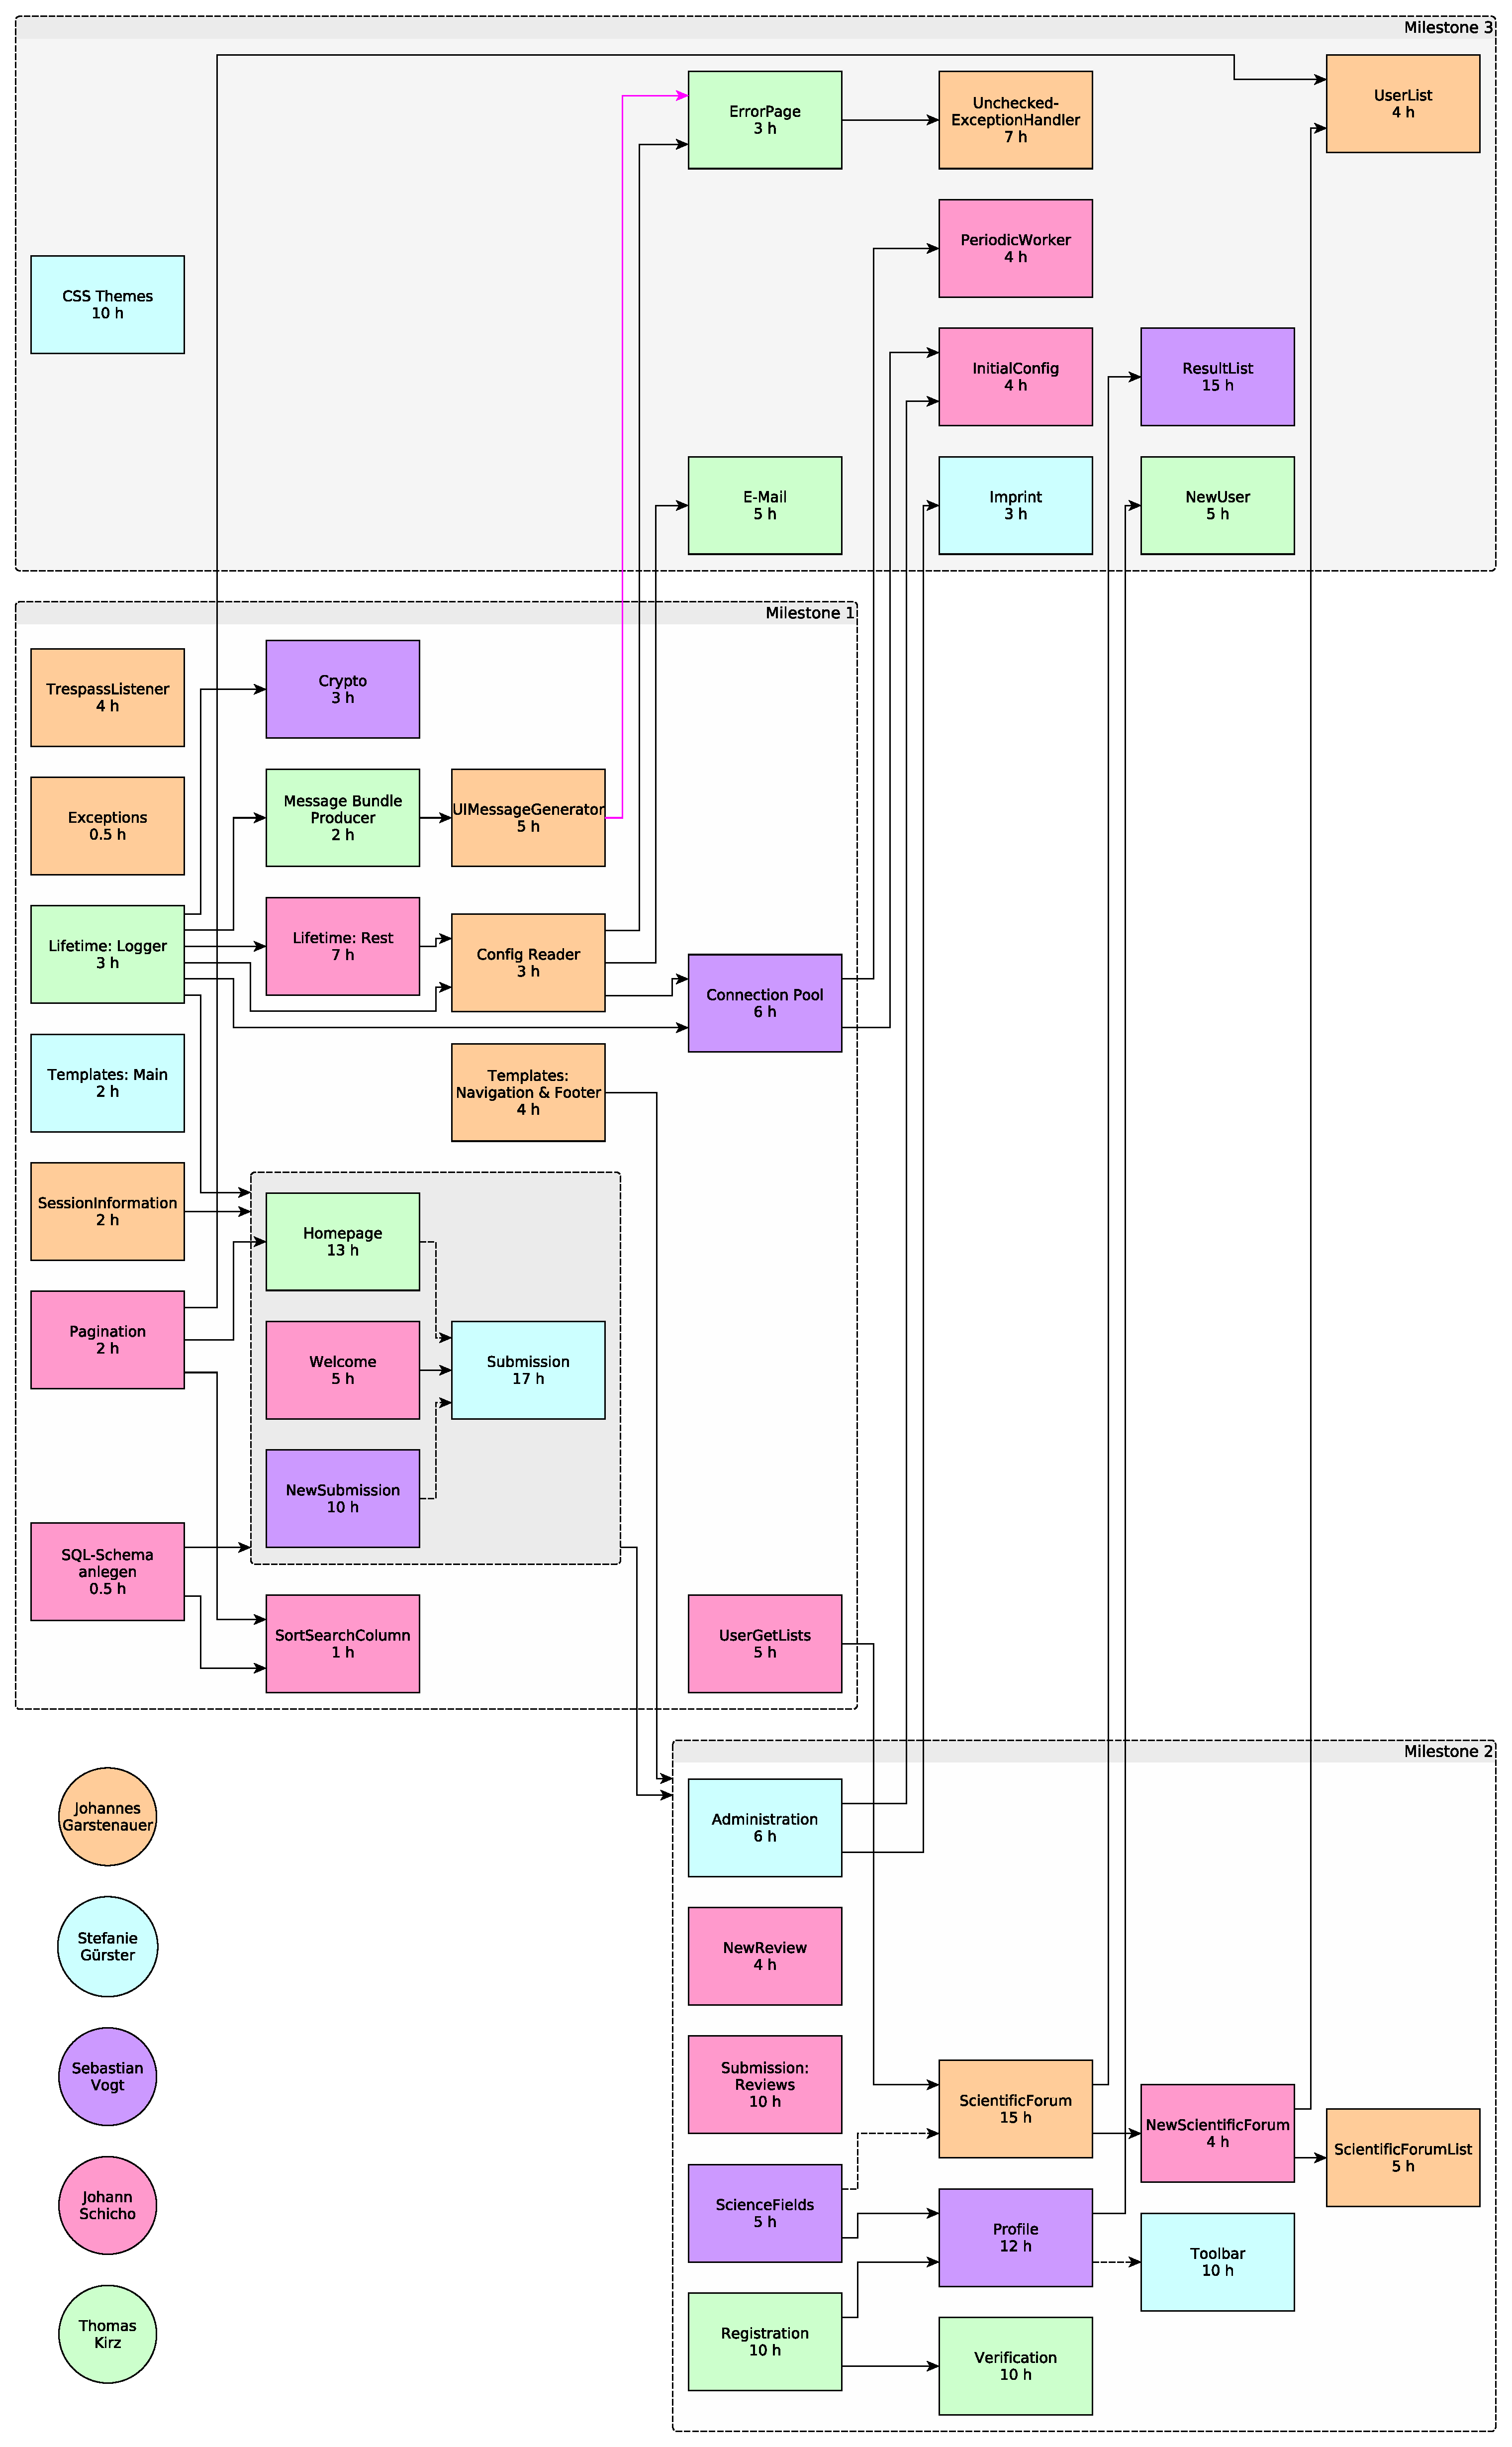
\includegraphics[width=\textwidth]{graphics/pert}
    \caption{Abhängigkeiten der Arbeitspakete in einem PERT-Chart}
    \label{fig:pert}
\end{figure}